\begin{block}{Continuum limit}
    We compute $\chi$ in units of the flow scale $t_0$, and we attempt a continuum limit.
    \begin{figure}
      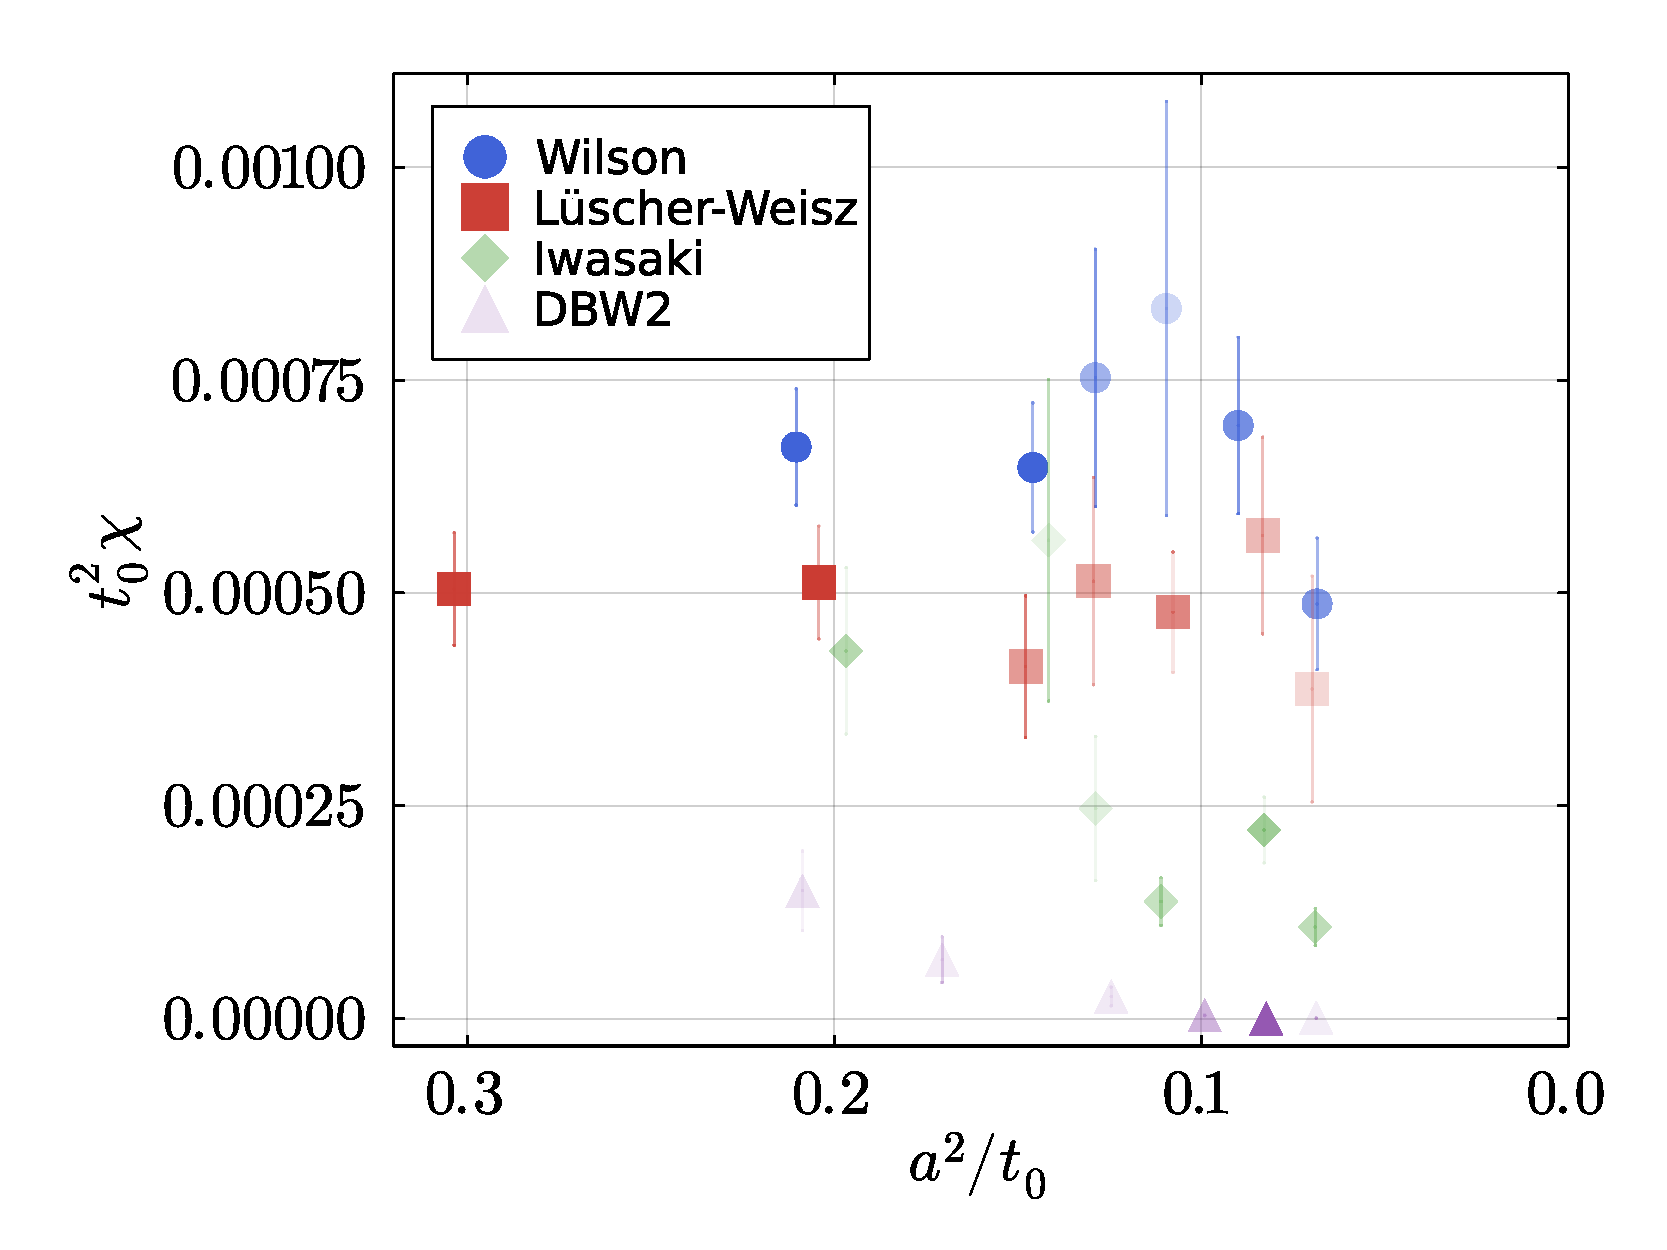
\includegraphics[scale=0.6]{PLOTS/L64_CL.pdf}
      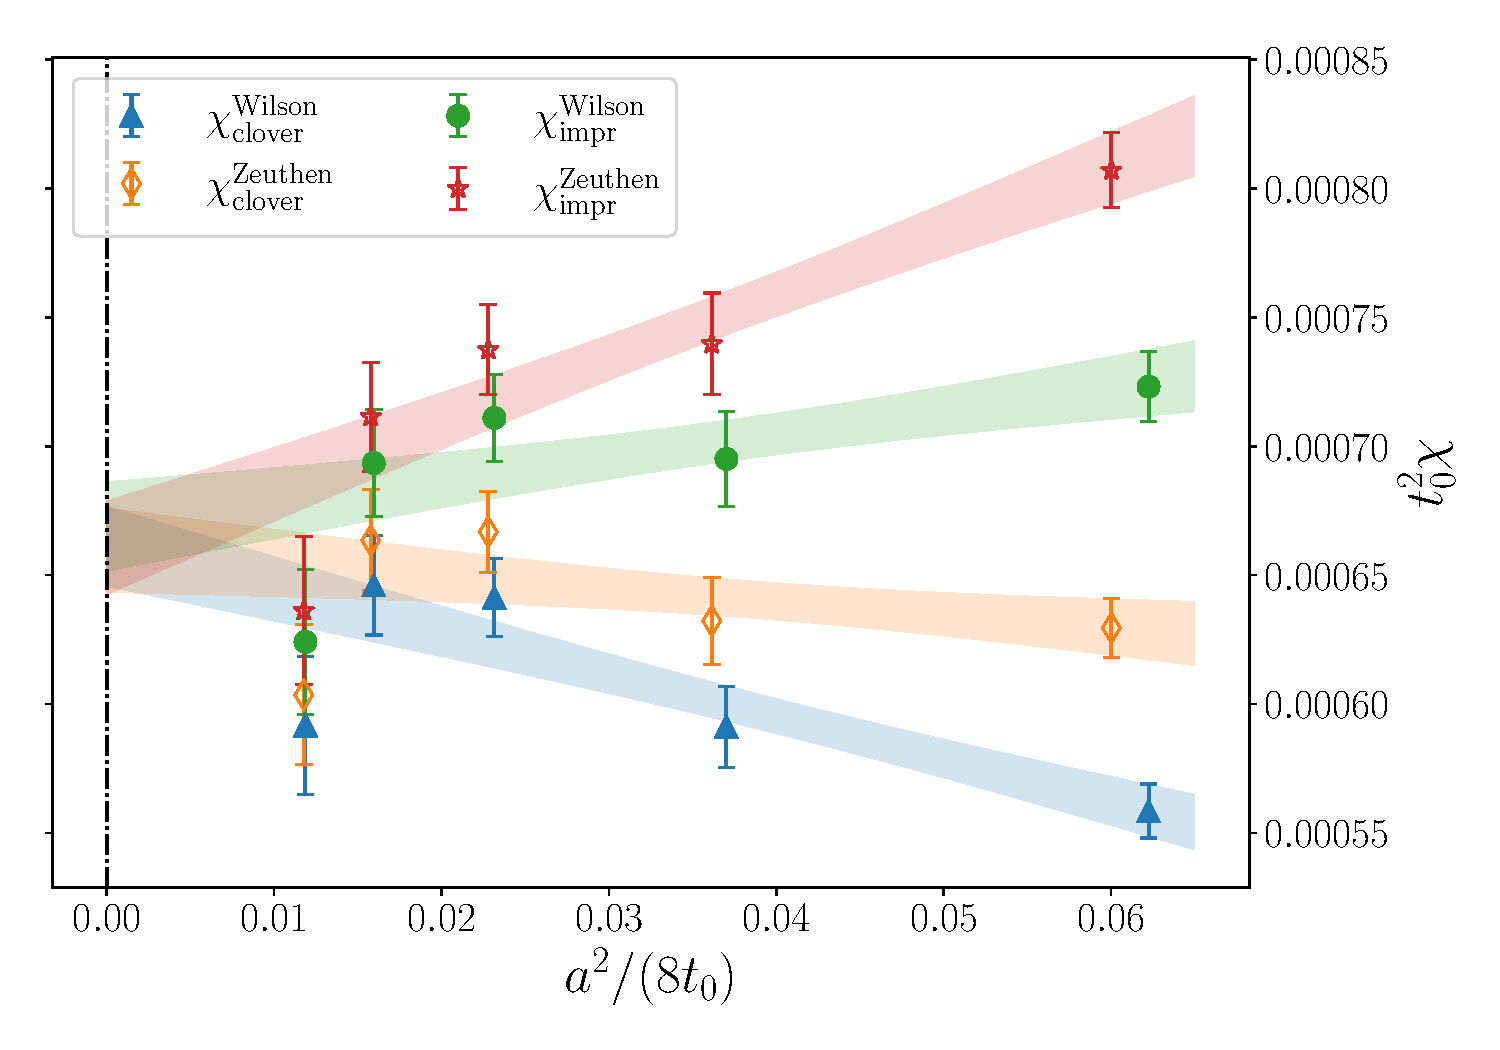
\includegraphics[scale=0.7]{PLOTS/cl_behaviour_t0.pdf}
    \end{figure}
    \begin{description}
        \item[\textbf{Left:}] The Iwasaki and DBW2 ensembles are effectively frozen — topology is suppressed and the charge is badly undersampled — so we attempt a continuum extrapolation only for Wilson and Lüscher-Weisz, whose limits agree.
        \item[\textbf{Right:}] 4 extrapolations from a single set of Lüscher-Weisz configurations with more statistics, spanning all combinations of Wilson/Zeuthen flow and clover/improved charge. The four definitions differ only at $\order{a^2}$ and, despite slopes of opposite sign, converge to a common continuum value — a nontrivial consistency check on the charge and flow discretisations.
    \end{description}
\end{block}